\section{Hidden Markov Models (HMM)}

\begin{frame} 
\mode<presentation>{
    \begin{center} \huge
        \secname
    \end{center}
    }    
    \begin{center}
    Latent variable model for temporal data.
    \end{center}
	
\end{frame}

\begin{frame}{\secname}

HMMs operate on the following Markov chain of the latent variables:
\begin{equation}
P(\vec{m}^{(t)}  ~|~ \vec{m}^{(1)},  \dots,\vec{m}^{(t-1)}) =
		P(\vec{m}^{(t)}  ~|~ \vec{m}^{(t-1)})
\end{equation}

and that $\vec x^{(t)}$ depends directly on $\vec m^{(t)}$

\begin{equation}
P(\vec{x}^{(t)}  ~|~ \vec{x}^{(1)},  \dots,\vec{x}^{(t-1)}, \vec{m}^{(1)},  \dots,\vec{m}^{(t)}) =
		P(\vec{x}^{(t)}  ~|~ \vec{m}^{(t)})
\end{equation}

We want to estimate the above densities in the graphical model that is the HMM.

\end{frame}

\begin{frame}{Recap: Latent variable models - the likelihood}

Latent variable models operate on the joint distribution of the observed and hidden variables.
The likelihood is recovered by \textcolor{blue}{marginalizing} the latent variable.
Recall in the general case of latent variable models:

\begin{equation}
P \left( \vec{x}^{(\alpha)} | \vec{w} \right) =
\kern-3.5ex
\underbrace{{\color{blue}\sum_{\vec{m}}}}_{
\substack{
\text{\tiny all possible}\\
\text{\tiny valid assignments}\\
\text{\tiny for point }\alpha}} 
\kern-3ex
P \left( \vec{x}^{(\alpha)}, \vec{m} | \vec{w} \right)
\end{equation}

\pause

\svspace{-5mm}

For HMMs\notesonly{ this would take the following shape}:

\svspace{-5mm}

\begin{equation}
P \left( \vec{x}^{(t)} |~\text{param.} \right) =
\kern-4ex
\underbrace{{\color{blue}\sum_{\vec{m}}}}_{
\substack{
\text{\tiny all possible}\\
\text{\tiny valid assignments}\\
\text{\tiny at step t}
}
}
\kern-3ex
P \left( \vec{x}^{(t)}, \vec{m}^{(t)} |~\text{param.} \right)
\stackrel{\substack{\text{for}\\
\text{brevity}}}{=}
{\color{blue}\sum_{\vec{m}}}
P \left( \vec{x}^{(t)}, \vec{m}^{(t)} \right)
\end{equation}

\pause

Next: Formulation of the joint distribution of the entire sequence

\pause

\question{What do we need this for?}

\notesonly{
-The optimization of the HMM boils down to maximizing the data likelihood. In this case the likelihood of the observed sequence. And for a latent variable model such as the HMM, this requires marginalization of the latent variables for all time steps in the sequence.
}

\end{frame}

\begin{frame}{The trellis diagram of the HMM}

\begin{center}
	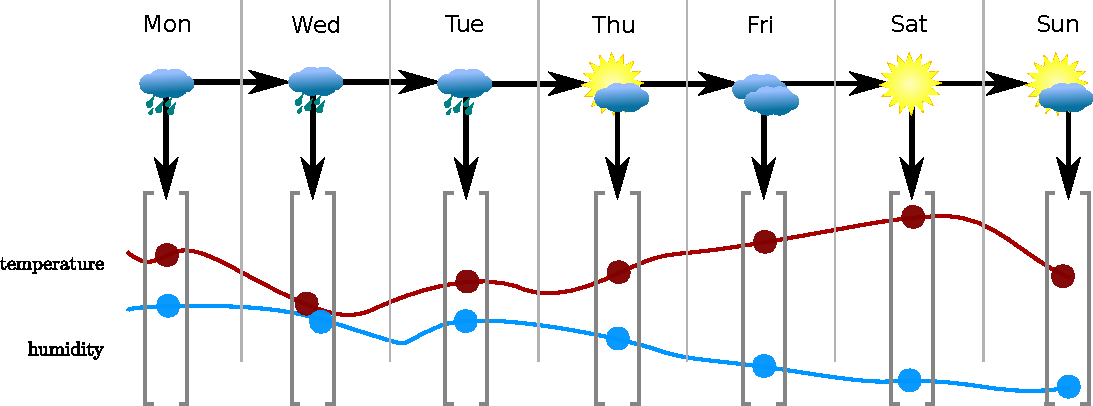
\includegraphics[width=0.8\textwidth]{img/weather_trellis}
	\notesonly{\captionof{figure}{The trellis diagram of the HMM depicting the dependencies between the variables.}}
\end{center}

\slidesonly{
We recognize the Markov properties in the \emph{trellis diagram} of the HMM
\begin{itemize}
\item
Every state $\vec{m}^{(t)}$ depends only on the previous state $\vec{m}^{(t-1)}$
\begin{equation}
P(\vec{m}^{(t)}  ~|~ \vec{m}^{(1)},  \dots,\vec{m}^{(t-1)}) =
		{P(\vec{m}^{(t)}  ~|~ \vec{m}^{(t-1)})}
\end{equation}

\item Every observation $\vec x^{(t)}$ depends only on $\vec m^{(t)}$

\begin{equation}
P(\vec{x}^{(t)}  ~|~ \vec{x}^{(1)},  \dots,\vec{x}^{(t-1)}, \vec{m}^{(1)},  \dots,\vec{m}^{(t)}) =
		{P(\vec{x}^{(t)}  ~|~ \vec{m}^{(t)})}
\end{equation}
\end{itemize}
}

\end{frame}

\begin{frame}{The factorization corresponding to the graphical model of the HMM}

\notesonly{The factorization corresponding to the graphical model of the HMM:}

\slidesonly{
From the Markov property in the HMM:
\begin{equation}
P(\vec{m}^{(t)}  ~|~ \vec{m}^{(1)},  \dots,\vec{m}^{(t-1)}) =
		{\color{magenta}P(\vec{m}^{(t)}  ~|~ \vec{m}^{(t-1)})}
\end{equation}

and that $\vec x^{(t)}$ depends directly on $\vec m^{(t)}$

\begin{equation}
P(\vec{x}^{(t)}  ~|~ \vec{x}^{(1)},  \dots,\vec{x}^{(t-1)}, \vec{m}^{(1)},  \dots,\vec{m}^{(t)}) =
		{\color{cyan}P(\vec{x}^{(t)}  ~|~ \vec{m}^{(t)})}
\end{equation}
}

\begin{block}{Conditional independence}
Two random variables $X$ and $Y$ are conditionally independent if:

\svspace{-3mm}

\begin{equation}
P(X,Y|Z) \;=\; P(X|Z) P(Y|Z).
\end{equation}

\svspace{-5mm}

Consequently,

\svspace{-3mm}

\begin{equation}
P(X,Y,Z) \stackrel{\substack{\text{product}\\\text{rule}}}{=} P(X,Y|Z)P(Z) \;=\; P(X|Z) P(Y|Z)P(Z).
\end{equation}
\end{block}

\notesonly{We exploit the Markov property to factorize the joint distribution for the observed and hidden sequences for the HMM:}

\svspace{-4mm}

\begin{align}
P(\{\vec{x}^{(t)}\}  , \{\vec{m}^{(t)}\}) = 
		P(\vec{m}^{(1)})
		\Bigg\lbrack
		\prod_{t=2}^T
		{\slidesonly{\color{magenta}}
		P(\vec{m}^{(t)} ~|~ \vec{m}^{(t-1)})
		}
		\Bigg\rbrack
		\prod_{t=1}^T 
		{\slidesonly{\color{cyan}}
		P(\vec{x}^{(t)} ~|~ \vec{m}^{(t)})
		}
\end{align}


\end{frame}

\subsection{Parameters of an HMM}

\definecolor{darkgreen}{rgb}{0,0.6,0}

\begin{frame}{\subsecname}

The parameters of an HMM are split into the following sets:
\begin{enumerate}
\item {Transition probabilities}:\\
The probability of going from state $q$ to $r$ \notesonly{(\sectionref{sec:hmm_transition})}
\item The initial distribution:\\
The probability of a state initiating a sequence.  \notesonly{(\sectionref{sec:hmm_init})}
\item Emission probabilities:\\
the distribution of observations given the hidden state $q$.  \notesonly{(\sectionref{sec:hmm_emission})}
\end{enumerate}

\end{frame}

\subsubsection{Transition model}
\label{sec:hmm_transition}

\begin{frame}{\subsubsecname}

Transition probabilities:\\

The probability of going from state $q$ to $r$:\\

\begin{equation}
	A_{qr}^{(t)} :=	P(m_r^{(t)} = 1 ~|~  m_q^{(t - 1)} = 1)
\end{equation}
\notesonly{Store all transition probabilities in a }transition probability matrix
\begin{equation}
	\vec A^{(t)} \in \lbrack 0, 1\rbrack^{M\times M} \quad \text{(stochastic matrix)}
\end{equation}
with $\sum_{r=1}^M A_{qr}^{(t)} = 1 \quad \forall q= 1, \dots, M$\\
Assuming homogeneity simplifies this by reducing the transitions to a single matrix $\vec A$ independent of time step t.

\pause

\begin{equation}
P(\vec{m}^{(t)} ~|~ \vec{m}^{(t - 1)}; \vec{A}) = \prod_{r=1}^M \prod_{q=1}^M A_{qr}^{m_q^{(t-1)} m_r^{(t)}}
\end{equation}

\end{frame}

\subsubsection{Initial distributions}
\label{sec:hmm_init}


\begin{frame}{\subsubsecname}

Initial distributions (considered part of the transition model):\\
The probability of the initial state is given by the distribution
\begin{equation}
P(\vec{m}^{(1)} ~|~ \vec{b}) = \prod_{q=1}^M b_q^{m_q^{(1)}}
\end{equation}
	parameterized by probability vector $\vec{b} \in [0, 1]^M$ 
	
	whose elements $b_q := P(m_q^{(1)} = 1)$ satisfy $\sum_{q=1}^M b_q = 1$

	($\leadsto ~ \vec{b}$ has $M-1$ degrees of freedom)
	
	\pause
	
	Example from text data:\\
	\begin{equation}
		P(\text{``}\text{Once upon a time}\text{''}) > P(\text{``}\text{lived happily ever after}\text{''})
	\end{equation}
	
	\svspace{5mm}
	
	$\leadsto$ transition model $\vec{m}^{(1)}$ and $\vec{m}^{(t-1)} \rightarrow \vec{m}^{(t)}$ for $t=2, \dots, T$
	
	\hspace{5mm} fully specified through parameters $\vec{A}$ and $\vec{b}$

\end{frame}


\begin{frame}{The transition model}

Given
\begin{itemize}
\item Transition probabilities
\slidesonly{$
	P(\vec{m}^{(t)} ~|~ \vec{m}^{(t - 1)}; \vec{A}) = \prod_{r=1}^M \prod_{q=1}^M A_{qr}^{m_q^{(t-1)} m_r^{(t)}}
$
	}
\item Initial distributions
\slidesonly{
$
P(\vec{m}^{(1)} ~|~ \vec{b}) = \prod_{q=1}^M b_q^{m_q^{(1)}}
$
}
\end{itemize}

\only<1>{

\question{What is the probability of a sequence of states ``$3, 1, 2, 5$''?}

}

\only<2>{
	%\svspace{-3mm}rrrrr

	1-out-of-$M$ coding implies:
	\begin{itemize}
	\item[] state ``\textcolor{blue}{3}'': $\vec m = (0, 0, {\color{blue}1}, 0, \ldots, 0)^\top$,
	\item[] state ``\textcolor{darkgreen}1'': $\vec m = ({\color{darkgreen}1}, 0, 0, 0, \ldots, 0)^\top$
	\end{itemize}

	\begingroup
	\small
	\begin{align}
		P(\text{``}3, &1, 2, 5\text{''} | \vec A,\vec b) = P(\text{``}3\text{''} | \vec b) P(\text{``}3, 1, 2, 5\text{''} | \vec A) \\
		&= b_3 \cdot A_{31} \cdot A_{12} \cdot A_{25} \\
		&=
		%\kern-7ex= 
		%{\tiny 
		P(\vec{m}^{(1)} |~ \vec{b}) \cdot 
		P(\vec{m}^{(2)} |~ \vec{m}^{({1})}; \vec{A}) \cdot P(\vec{m}^{(3)} |~ \vec{m}^{(2)}; \vec{A}) \cdot P(\vec{m}^{(4)} |~ \vec{m}^{(3)}; \vec{A})
	\end{align}
	\endgroup
}

\only<3>{

\svspace{5mm}

	The probability of a sequence $\{\vec m^{(t)}\}$ in general:

	\begingroup
	\small
	\begin{align}
		P(\{\vec m^{(t)}\} ~|~ \vec A, \vec b) = P(\vec{m}^{(1)} |~ \vec{b}) \cdot \prod_{t={\color{red}2}}^{T} P(\vec{m}^{(t)} ~|~ \vec{m}^{({\color{red}t - 1})}; \vec{A})
	\end{align}
	\endgroup
}
\end{frame}

\subsubsection{Emission model}
\label{sec:hmm_emission}


\begin{frame}{\subsubsecname}

Emission probabilities $P(\vec x^{(t)} | \vec m^{(t)} ; \vec \phi)$

Where $\vec \phi = \{\vec \phi_1, \ldots, \vec \phi_M\}$ specifies the parameters of the set of $M$ components.

Analogous to mixture components $P(\vec x| q)$ of a mixture model, e.g. choosing Gaussian basis functions
\begin{equation}
P(\vec{x} ~|~ \vec{m}; \vec{\boldsymbol{\phi}}) = \prod_{q=1}^M
	P(\vec{x}^{(t)} ~|~ \vec{\boldsymbol{\phi}}_q)^{m_q^{(t)}} := \prod_{q=1}^M \mathcal{N}^{m_q} (\vec{x} ~|~ \vec{\boldsymbol{\mu}}_q, \vec{\Sigma}_q)
\end{equation}
				
where $\vec{\boldsymbol{\phi}} := \big\{\underbrace{\vec{\boldsymbol{\mu}}_q, \vec{\Sigma}_q}_{\vec{\boldsymbol{\phi}}_q} \big\}_{q=1}^M$

Example:\\
\begin{equation}
P(\mathit{temperature}=29^{\circ}, \mathit{humidity}=20\% ~|~ \text{``}\mathit{cloudy}\text{''}; \vec \phi)
\end{equation}

\end{frame}

%%%%%%%%%%%%%%%%%%%%%%%%%%%%%%%%%%%%%%%%%%%%%%%%%%%%%%%%%%%%%%%%%%%%%%
\begin{frame}{The parameterized HMM}
	
A more detailed specification of the joint distribution becomes:
	
	\begin{align}
	&P(\{\vec{x}^{(t)}\}  , \{\vec{m}^{(t)}\} ~|~ \vec{w})
	 \\&
	~=P(\vec{m}^{(1)})
	\Bigg\lbrack
	\prod_{t=2}^T
	P(\vec{m}^{(t)} ~|~ \vec{m}^{(t-1)})
	\Bigg\rbrack
	\prod_{t=1}^T P(\vec{x}^{(t)} ~|~ \vec{m}^{(t)})
	\\&~=
	\underbrace{P(\vec{m}^{(1)}~|~ \vec{b})}_{\text{initial hidden state}}
	\prod_{t=2}^{T} 
		\underbrace{P(\vec{m}^{(t)}~|~  \vec{m}^{(t - 1)},~ \vec{A})
		}_{\text{transition to next hidden state}}
	\prod_{t=1}^{T} 
	\underbrace{P(\vec{x}^{(t)}~|~  \vec{m}^{(t)},~ \vec{\boldsymbol{\phi}})
	}_{\text{emission model $\leadsto$ observation}}
	\end{align}
	
	where $\vec{w} := \{ 
	\kern-3.5ex
		\underbrace{\vec{A}}_{\substack{\text{state transition} \\ \text{probabilities}}}, \underbrace{\vec{b}}_{\substack{\text{initial state} \\ \text{probabilities}}}, \underbrace{\vec{\boldsymbol{\phi}}}_{\substack{\text{emission} \\ \text{components}}} 
	\kern-2.5ex
		\}$ summarizes the model parameters
	
\end{frame}
%%%%%%%%%%%%%%%%%%%%%%%%%%%%%%%%%%%%%%%%%%%%%%%%%%%%%%%%%%%%%%%%%%%%%%
